
\documentclass[12pt]{article}
\usepackage[a4paper, margin=.30in]{geometry}
\usepackage{graphicx ,
            wrapfig,
            xcolor, 
            enumerate,
            amsmath,
			fontenc,
			tcolorbox,circuitikz,tikz,bm
            }

%\usepackage{scalerel}
%\usepackage{pict2e}
%\usepackage{tkz-euclide}
%\usetikzlibrary{calc}
%\usetikzlibrary{patterns,arrows.meta}
%\usetikzlibrary{shadows}
%\usetikzlibrary{external}

%%pgfplots
\usepackage{pgfplots}
%\pgfplotsset{compat=newest}
%\usepgfplotslibrary{statistics}
%\usepgfplotslibrary{fillbetween}

\newcommand\headerMe[2]{\noindent{}#1\hfill#2}
\renewcommand{\thesection}{\Roman{section}}

\author{Zakaria HAOUZAN}
\date{\today}

\begin{document}
% headers --------------
\headerMe{Matière : Physique-Chimie}{Professeur : Zakaria HAOUZAN}\\
\headerMe{Unité : Mécanique }{Établissement : Lycée SKHOR qualifiant}\\
\headerMe{Niveau : 2BAC-SM-PC}{Heure : 5H}\\

% ------Content ________
\begin{center}

    \Large{Leçon $N^{\circ} 10 $: \color{red}Les loi de Newton}
\end{center}

%\begin{wrapfigure}[10]{r}{0.5\textwidth}
%    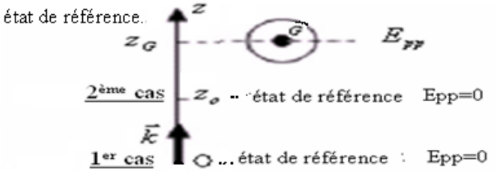
\includegraphics[width=0.5\textwidth]{./img/img00.png}
%\end{wrapfigure}


\section{Vecteur vitesse- vecteur accélération}
\subsection{Notions générales sur le mouvement:}

\begin{wrapfigure}[1]{r}{0.3\textwidth}
	\vspace{-5cm}
\begin{tikzpicture}[scale=1.4]
\draw (0,0) --++ (1,1) --++ (3,0) --++ (-1,-1) --++ (-3,0);
\draw [thick] [->] (2,0.5) --++(0,2) node [right] {z};
%thick : gras ; very thick : très gras ; ultra thick : hyper gras
\draw (2,0.5) node [left] {O};
\draw [thick] [->] (2,0.5) --++(-1,-1) node [left] {x};
\draw [thick] [->] (2,0.5) --++(2,0) node [below] {y};
\end{tikzpicture}
\end{wrapfigure}
Nous savons que le mouvement d'un corps est relatif au référentiel choisi, c'est-à-dire que les corps ne se déplacent
que par rapport à d'autres corps.
Donc pour étudier le mouvement d'un corps on doit choisir un solide de réference fixe appelé référentiel puis un repère d'espace et un repère de temps liés à ce referential.

\begin{tcolorbox}
Remarque: la plupart des temps, on choisi comme référentiel d'étude le référentiel terrestre.
Pour repérer la position du mobile, on utilise un repère d'espace $(O,\vec{i} , \vec{j}, \vec{k} )$
d'origne O et dont les vecteurs unitaires: $\vec{i} , \vec{j}$ et  $\vec{k}$.

Le vecteur Position : $\vec{OG} = x.\vec{i}+y.\vec{j}+z.\vec{k}$

G: Centre d'inertie du corps

x,y et z :sont les coordonnée du centre d'inertie G dans le repère $(O,\vec{i} , \vec{j}, \vec{k} )$

Si le corps est en mouvement, ses coordonnées x,y et z variant en fonction du temps


Les fonctions : $x=f(t)$ , $y=g(t)$ et $h(t)$ sont appelées les équations horaires du mouvement.

La trajectoire est l'ensemble des positions successives occupées par le mobile au cours de son mouvement.
\end{tcolorbox}

\subsection{Le vecteur vitesse instantanée:}
\subsubsection{Définition:}
Le vecteur vitesse instantanée du centre d'inertie d'un corps est égal à la dérivée du vecteur position par rapport au
temps. $$\vec{v}_G = \frac{d\vec{OG}}{dt}$$
\subsubsection{Les coordonnées du vecteur vitesse dans un repère cartésien:}
avec : $\vec{v}_G = \frac{d\vec{OG}}{dt} = \frac{x}{dt}.\vec{i} + \frac{y}{dt}.\vec{j} + \frac{z}{dt}.\vec{k}$  et -----------  $\vec{v}_G = v_x.\vec{i} + v_y.\vec{j} + v_z.\vec{k}$ avec ----- $v_x = \frac{x}{dt} = \dot{x}$
-----$v_y = \frac{y}{dt} = \dot{y}$
-----$v_z = \frac{z}{dt} = \dot{z}$
Le module du vecteur vitesse: $v_G = ||\vec{v_G}|| = \sqrt{\dot{x}^2 + \dot{y}^2 + \dot{z}^2 }$

\subsection{Le vecteur accélération:}
\subsubsection{Définition:}
Le vecteur accélération du centre d'inertie d'un corps est égal à la dérivée du vecteur vitesse par rapport au temps.
 $$\vec{a_G} = \frac{d\vec{v_G}}{dt}$$

\subsubsection{Les coordonnées du vecteur accélération dans un repère cartésien:}
avec : $\vec{a}_G = \frac{d\vec{v_{OG}}}{dt} = \frac{v_x}{dt}.\vec{i} + \frac{v_y}{dt}.\vec{j} + \frac{v_z}{dt}.\vec{k}$  et -----------  $\vec{v}_G = a_x.\vec{i} + a_y.\vec{j} + a_z.\vec{k}$ avec ----- $a_x = \frac{v_x}{dt} = \ddot{x}$
-----$a_y = \frac{v_y}{dt} = \ddot{y}$
-----$a_z = \frac{v_z}{dt} = \ddot{z}$
Le module du vecteur vitesse: $v_G = ||\vec{v_G}|| = \sqrt{\ddot{x}^2 + \ddot{y}^2 + \ddot{z}^2 }$


\subsubsection{Les coordonnées du vecteur accélération dans un repère de Frenet:}
Le repère de Frenet est un repère local orthonormé lié au mobile que l'on note $(M,\vec{u},\vec{n})$
, le vecteur unitaire $\vec{u}$
est tangent à la trajectoire au point M et orienté dans le sens du mouvement.
Le vecteur unitaire $\vec{n}$
est normal, et dirigé vers le centre de courbure de la trajectoire, il est perpendiculaire à $\vec{u}$

\begin{itemize}
	\item L'expression du vecteur accélération dans le repère de Frenet est: $\vec{a_G} = a_t.\vec{u} + a_n.\vec{n}$

	\item $a_t = \frac{dv}{dt}$ : la composante tangentielle du vecteur accélération
	\item $a_n = \frac{v^2}{R}$ : la composante normale du vecteur accélération
	\item R : : est le rayon de courbure de la trajectoire au point M.
\end{itemize}

\section{Les Lois de NewTon : }
\subsection{Les forces intérieures et les forces extérieures:}
Après avoir précisé le système étudié :
\begin{itemize}
	\item On appelle forces extérieures, les forces qui s'exercent sur le système par des corps qui n'appartiennent pas au système.
	\item On appelle forces intérieures, les forces qui s'exercent sur le système par des corps qui appartiennent pas au système.

\end{itemize}
\begin{tcolorbox}
Remarque: Un système est dit isolé s'il n'est soumis à aucune force extérieure.
Un système est dit pseudo-isolé si les force extérieure auquel il est soumis se compensent.
\end{tcolorbox}


\subsection{La première loi de Newton :Principe d'inertie:} 
Dans un repère galiléen, si la somme des forces qui s'exercent sur un corps est nulle, alors le vecteur vitesse de son centre
d'inertie est constant. $\sum \vec{F} = \vec{0}$ $\rightarrow$ $\vec{V_G} = C^{te}$

Donc le centre d'inetie du corps est:
-Soit au repos. \hspace{2cm }- Soit en mouvement rectiligne uniforme.

\subsection{La deuxième loi de Newton:}
Dans un repère galiléen la somme des vecteurs forces qui s'exercent sur un corps est égale au produit de la masse du
corps et du vecteur accélération de son centre d'inertie.$$\sum \vec{F_{ext}} = m.\vec{a_G}$$

\subsection{La troisième loi de Newton : principe de l'action et de la réaction.}

Lorsqu'il y'a interaction entre deux corps A et B , le corps A exerce une force $\vec{F_{A/B}}$ sur le corps B et le corps B exerce une force $\vec{F_{B/A}}$ sur le corps A ,ces deux forces sont telles que: $\vec{F_{A/B}} = -\vec{F_{A/B}}$


\section{Le mouvement rectiligne uniforme et le Mouvement rectiligne uniformément varié M}

Généralement le repère utilisé pour étudier les mouvement rectiligne est un axe (O,x) confondu avec la trajectoire et orienté
dans le sens du mouvement et dans ce cas le vecteur position $\vec{OG} = x.\vec{i}$ et la vitesse du mobile $v = \frac{dx}{dt}$ et son accélération $a =\dot{v}=\ddot{x}$

\subsection{Le mouvement rectiligne uniforme : } 
Le mouvement rectiligne uniforme est caractérisé par :

\begin{itemize}
	\item Une trajectoire rectiligne .
	\item Une accélération nulle a=0.
	\item Une vitesse constante v=Cte
	\item L'équation horaire du mouvement est : $x = v.t+x_0$ (avec $x_0$: abscisse à l'origine)

\end{itemize}

\subsection{Le mouvement rectiligne uniformément varié : }

\begin{itemize}
	\item Une trajectoire rectiligne .
	\item  Une accélération constante a=Cte
	\item L'équation horaire du mouvement est : $x = \frac{1}{2}.a.t^2 + v_0.t+ x_0$ (avec $ x_0$: abscisse à l'origine).
	\item L'équation de la vitesse : $v = a.t + v_0$
	\item Dans ce cas la vitesse en fonction du temps est une fonction affine, son coefficient directeur est égal à l'accélération.
\end{itemize}


\section{Application :}
En général la 2ème loi de Newton sert à déterminer la nature du mouvement du centre d'inertie d'un mobile connaissant les
forces qui s'appliquent sur lui.
Pour résoudre un problème de dynamique en utilisant la deuxième loi de Newton on doit toujours suivre les étapes suivantes:
\begin{enumerate}
	\item  On précise le système étudié.
	\item  On fait le bilan des forces extérieures qui s'exercent sur ce système.
\item  On représente ses forces.
\item  On écris la relation vectorielle de la 2ème loi de Newton $\sum \vec{F} = m.\vec{a_G}$.

\item  Puis on projète cette relation après avoir choisi un repère orthonormé convenable lié à un référentiel Galiléen.
\end{enumerate}


%wfg---------------------------------------------------------------sf 
%\begin{center}
   %\begin{tabular}{ |c|c|c|c|c|c|c| }
      %\hline
      %km & hm & dam & \bf{m} & dm & cm & mm \\
      %\hline
        %&   &    &  &   &   & \\
%\hline
%\end{tabular}
%On place un seul nombre dans chaque case.
%\end{center}
%\begin{center}
   %\begin{tabular}{ |c|c|c|c|c|c|c| }
      %\hline
      %$km^2$ & $hm^2$ & $dam^2$ & \bf{$m^2$} & $dm^2$ & $cm^2$ & $mm^2$ \\
      %\hline
        %&   &    &  &   &   & \\
%\hline
%\end{tabular}
%\end{center}


\end{document}

